\documentclass[12pt]{article}

% Packages
\usepackage{graphicx}
\usepackage{subcaption}
\usepackage{hyperref}
\usepackage{enumitem}
\usepackage{scrextend}

\usepackage[margin=1in]{geometry}

\usepackage[style=numeric,maxbibnames=99,sorting=none]{biblatex}
\addbibresource{tex/publications.bib}
\DeclareNameAlias{default}{given-family}

% Change how each biblatex bib heading is printed
\defbibheading{bibliography}[\refname]{%
  \subsubsection*{\normalfont\textit{#1}}%
}

% No translations, only English
\newcommand{\email}{joel.oskarsson@outlook.com}
\newcommand{\cvheading}[1]{\subsection*{#1}}

\graphicspath{{./graphics/}}

\pagenumbering{gobble}
\usepackage[utf8]{inputenc}

\begin{document}

\begin{figure*}
    \begin{subfigure}[]{0.3\textwidth}
        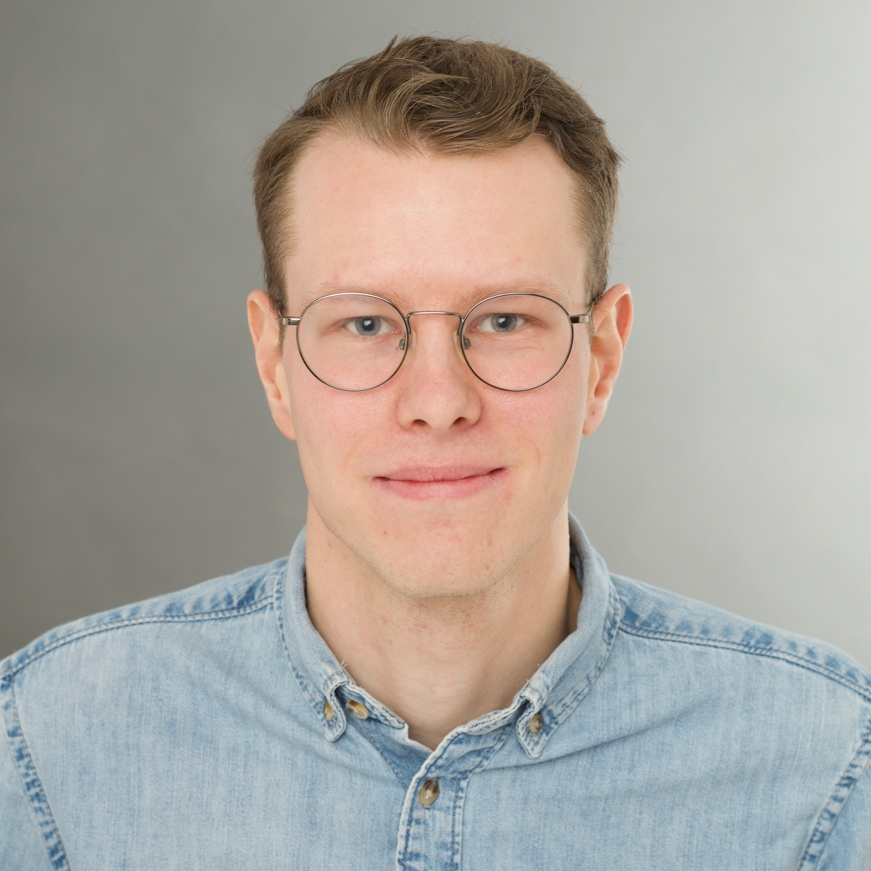
\includegraphics[height=5cm]{photo}
    \end{subfigure}%
    ~
    \begin{subfigure}[]{0.5\textwidth}
        \part*{Joel Oskarsson}

        \begin{tabular}{l l}
            \href{mailto:\email}{\email} & +46706724739\\
            \href{http://joeloskarsson.github.io}{joeloskarsson.github.io} & \href{http://linkedin.com/in/joel-oskarsson}{linkedin.com/in/joel-oskarsson}\\
        \end{tabular}
        \\
        \\

        \begin{tabular}{l l}
            Ebbegatan 18 & \\
            581 83, Linköping & \\
            Sweden & \\
        \end{tabular}

     \end{subfigure}%
\end{figure*}

\cvheading{Research Interests} %TODO
In my research I develop machine learning methods for data with spatial-, temporal- and graph-structure, including combinations of these.
I am interested in how more traditional probabilistic methods in these domains can be combined with deep learning in order to derive new methods with useful properties.
When evaluating and applying these methods to real-world problems I focus on applications within transport and vehicle systems as well as climate and weather modeling.

\cvheading{Education}
\begin{labeling}{2020--2025}
    \item [2020--2025] In progress: \textbf{Doctoral Studies in Computer Science, Linköping University}, Linköping, Sweden, 240 ECTS
        \begin{itemize}
            \item At the Division of Statistics and Machine Learning (STIMA), Department of Computer and Information Science. Supervised by \href{https://lindsten.netlify.app/}{Fredrik Lindsten} (main supervisor), \href{https://scholar.google.se/citations?user=0UomzRIAAAAJ}{Per Sidén} and \href{https://www.smhi.se/en/research/research-departments/meteorology/tomas-landelius-1.4817}{Tomas Landelius}.
            \item Title of PhD thesis: \textit{Graph-based Machine Learning for Spatio-Temporal Data (preliminary)}.
            Planned defense May 2025.
            \item Affiliated PhD Student in the \href{https://wasp-sweden.org/}{Wallenberg AI, Autonomous Systems and Software Program (WASP)}
        \end{itemize}
    \item [2015--2020]
            \textbf{Master's program in Computer Science and Engineering (Swedish Civilingenjörsprogram), Linköping University}, Linköping, Sweden, 300 ECTS
        %Aug 2015 -- June 2020
        \begin{itemize}
            \item Master's thesis: \href{http://urn.kb.se/resolve?urn=urn:nbn:se:liu:diva-166637}{Probabilistic Regression using Conditional Generative Adversarial Networks}
            \item \textbf{Exchange Year, ETH Zürich}, Zürich, Switzerland\\
        Sep 2018 -- Aug 2019\\
            First year of my master's as an exchange student at ETH. Courses mainly in machine learning and AI.
        \end{itemize}
\end{labeling}

\cvheading{Employment}
\begin{labeling}{2018, Summer}
    \item [2020 --]\textbf{PhD Student, Linköping University}, Linköping\\
        Research + 20\% of employment teaching.
    \item [2016--2019] \textbf{Teaching Assistant, Linköping University}, Linköping, Sweden\\
        Multiple periods.

    \item [2018, Summer] \textbf{Summer Intern, Ericsson}, Linköping, Sweden\\
        Internship at Ericsson Research, working with GNSS positioning.
\end{labeling}

\cvheading{Publications}
\nocite{*}
\printbibliography[keyword={journal},title={Journal papers}]
\printbibliography[keyword={conference},title={Peer-reviewed conference papers}]
\printbibliography[keyword={workshop},title={Peer-reviewed workshop papers}]
\printbibliography[keyword={preprint},title={Preprints}]

\cvheading{Research Presentations}
\textit{Invited talks}
\begin{labeling}{2024-01-01}
    \item [2024-08-22] Graph-based Machine Learning for Weather, European Centre for Medium-Range Weather Forecasts (ECMWF), Bonn, Germany.
    \item [2024-05-02] Graph-based Neural Weather Prediction for Limited Area Modeling, MeteoSwiss, Zürich, Switzerland.
    \item [2024-04-30] Graph-based Neural Weather Prediction for Limited Area Modeling, ETH Zürich, Zürich, Switzerland.
    \item [2024-04-17] Graph-based Machine Learning for Spatio-Temporal Data, with Application to Traffic and Weather Forecasting, University of New South Wales (UNSW), Sydney, Australia (Online).
    \item [2024-03-05] Graph-based Neural Weather Prediction for Limited Area Modeling, Uppsala University, Uppsala, Sweden.
    \item [2024-01-11] Neural Weather Prediction for Limited Area Modeling, IEA Wind Task 51 Webinar: Forecasting for the Weather Driven Energy System (Online).
    \item [2023-10-10] Graph-based Neural Weather Prediction for Limited Area Modeling, Danish Meteorological Institute, Copenhagen, Denmark.
\end{labeling}
\textit{Additional workshop presentations}

In addition to presentations of publications listed above, at publication venue.
\begin{labeling}{2023-06-22}
    \item [2024-08-29] Probabilistic Weather Forecasting with Hierarchical Graph Neural Networks, Large-Scale Deep Learning for the Earth System Workshop, Bonn, Germany.
    \item [2024-05-09] A Graph-Based Latent Variable Model for Probabilistic Weather Forecasting, ESA-ECMWF workshop on Machine Learning for Earth System Observation and Prediction, Frascati, Italy.
    \item [2023-09-04] GraphCast for a Limited Area Numerical Weather Prediction Model, Large-Scale Deep Learning for the Earth System Workshop, Bonn, Germany.
    \item [2023-06-22] Bayesian Learning on Graphs using Deep Gaussian Markov Random Fields, NORDSTAT Conference, Gothenburg, Sweden.
\end{labeling}

\cvheading{Teaching and Supervision}
    Apart from my research, I spend 20\% of my PhD student employment on teaching. Teaching activities include (all at Linköping University):
    \begin{itemize}
        \item Supervisor of 7 master's theses (2021--2024)
        \item Co-developer of the online course \href{https://foundations-of-ml.ida.liu.se/}{\textit{Foundations of Machine Learning}} (2021--2024)
        \item Pedagogical training course, \textit{Becoming a Teacher in Higher Education}, 6 ECTS (2021)
        \item Teaching assistant in courses (2016--2024):
            Advanced Machine Learning (5 occasions),
            Introduction to Python,
            Computational Statistics,
            Foundations of Machine Learning,
            Building AI,
            Machine Learning for Industry,
            Concurrent and Operating Systems Programming,
            Introductory Course in Calculus,
            Discrete mathematics (2 occasions)
            %Assisting and correcting labs in courses on machine learning, computational statistics and python programming.
    \end{itemize}

\cvheading{Other activities}
\begin{itemize}
    \item Regularly act as reviewer for established machine learning conferences and associated workshops. Including:
        AISTATS,
        ICLR,
        NeurIPS.
    \item Organizer of the \href{https://github.com/STIMALiU/ml-reading-group}{STIMA Machine Learning Reading Group} at Linköping University (2022--)
    \item Research visits, long and short (UCL, ECMWF, ETH/Meteoswiss, WASP finland trip?)
    \item Regular attendance at international conferences and workshops within machine learning.
    \item Media coverage https://www.svt.se/nyheter/lokalt/ost/de-vill-gora-vaderprognoser-mer-palitliga-med-hjalp-av-ai
    \item Creator and maintainer of the \href{https://github.com/mllam/neural-lam}{Neural-LAM} open source python library for machine learning weather forecsating models.
    \item ML-LAM online meetups
\end{itemize}

\cvheading{Specific Skills and Knowledge}
\begin{itemize}
    \item Extensive knowledge of models and algorithms for modern \textbf{machine learning and AI} applications. Specific expertise in:
    \begin{itemize}
        \item Graph neural networks
        \item Bayesian models and inference methods
        \item Probabilistic deep learning
    \end{itemize}

\item Sound knowledge of good \textbf{software engineering} practices, acquired from courses and projects throughout my undergraduate studies.
        % I apply these practices to my research projects, creating accessible code.
        % To emphasize transparency and reproducability in research I have made a habit to release research code publicly (see \href{my github page}{https://github.com/joeloskarsson}).

    \item Programming languages and frameworks
    \begin{description}
        \item [Knowledgeable in] Python, PyTorch, PyTorch Geometric and SciPy/NumPy.
        \item [Experience with] R, Tensorflow, scikit-learn, Java, MATLAB and C++.
    \end{description}

\item Highly accustomed to working in \textbf{Linux} environments.
\end{itemize}

\end{document}
